\Chapter{Tervezés}
Ebben a fejezetben a webalkalmazás kinézetéről és adatmodelléről lesz szó.


\Section{A feladatom}

A feladatom egy olyan webalkalmazás fejlesztése, amely alkalmas más oldalak autó hirdetéseinek aggregálására és az autók böngészésére. Az alkalmazás funkciói a követke-
zők:

\begin{itemize}
\item Regisztráció: a felhasználó végzi el felhasználónév és jelszó pár megadásával.
\item Jogosultságok:
	\begin{itemize}
	\item Admin: mindenhez hozzáfér, ő frissíti az elérhető autókat, felhasználók jogo-
sultságát változtatja, és törölheti a felhasználót.
	\item User: a hirdetések és a statisztika megtekintésére jogosult.
	\end{itemize}
\item Hirdetések megtekintése: Az oldalon megtalálható autókat tudjuk megtekinteni.
\end{itemize}

\Section{Kinézet és felépítés}

A kinézet minél felhasználóbarátabb lesz, ami azt jelenti, hogy lesz egy grafikus felhasz-
nálói felület ami úgy lesz kialakítva, hogy felhasználók minél könnyebben tudják majd használni az alkalmazást, könnyen átlátható legyen számukra.

A terveséhez az Uizard \cite{uizard} nevű oldalt használtam.

\subsection{Regisztráció és bejelentkezés}

Ha már van fiókunk az oldalhoz, akkor a felhasználónév és a jelszó megadása után be is tudunk jelentkezni az oldalra (\ref{fig:Bejelentkezés}. ábra). Ha rossz felhasználónevet vagy jelszót adunk meg, akkor a következő értesítést fogjuk kapni: "Rossz felhasználónév vagy jelszó!".

\newpage

\begin{figure}[h]
\centering
\fbox{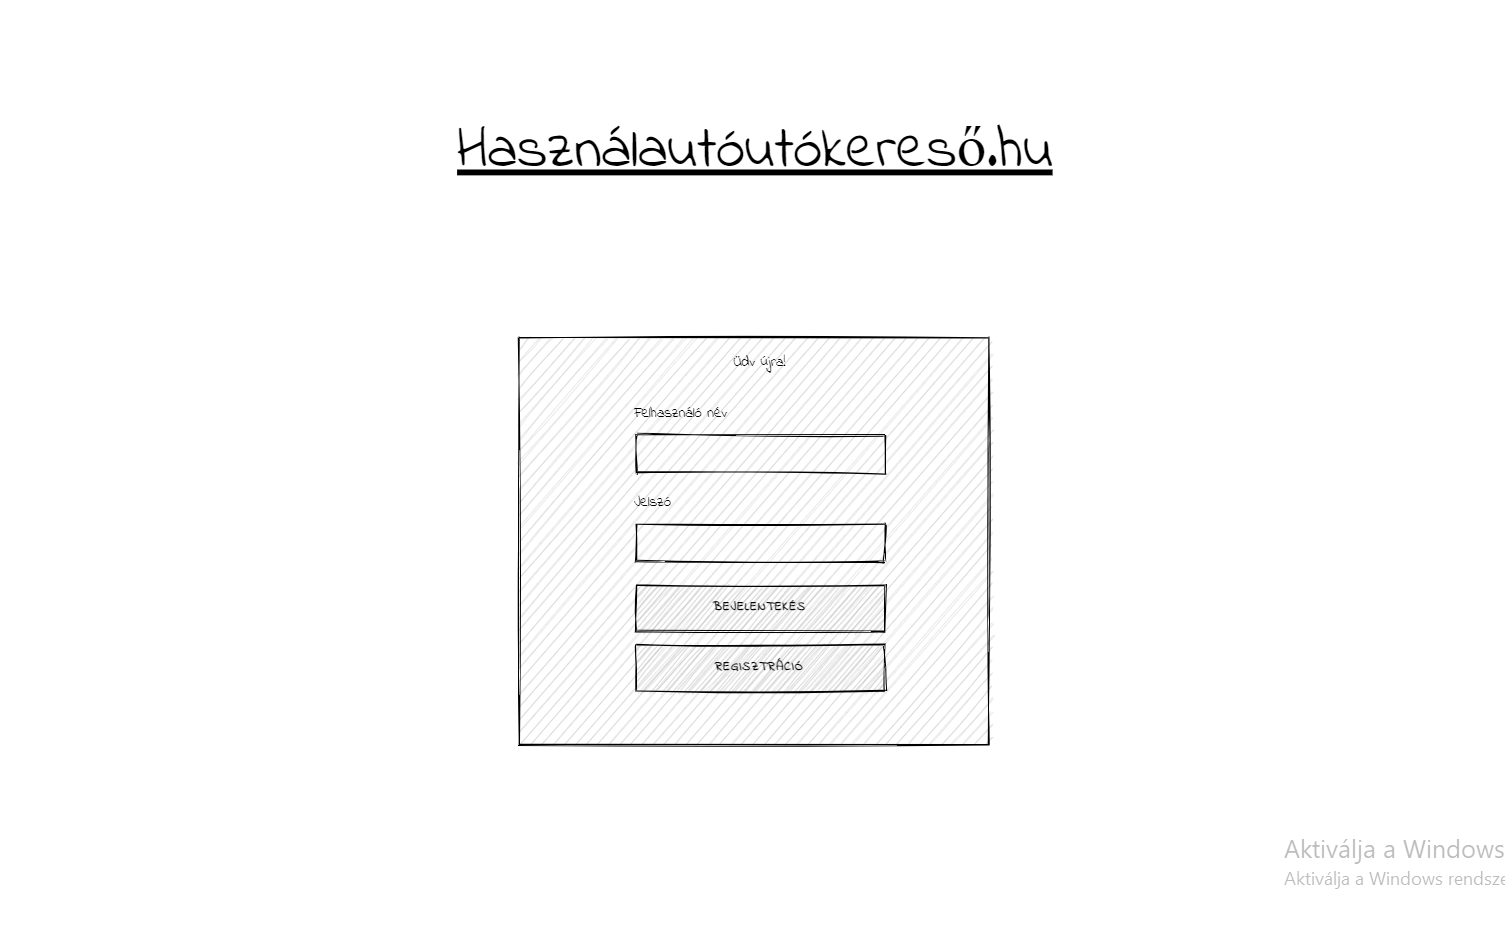
\includegraphics[scale=0.4]{images/login.png}}
\caption{Bejelentkezés}
\label{fig:Bejelentkezés}
\end{figure}

A regisztrációs felületen a felhasználónév és jelszó megadása után be tudunk regiszt-
rálni (\ref{fig:Regisztráció}. ábra), és máris tudjuk használni a weboldalt.

Ha nem adunk meg jelszót vagy felhasználó nevet, akkor arról majd értesítést fogunk kapni, ami a következő lesz: "Valamelyik mezőt kitöltetlenül hagyta!".

\begin{figure}[h]
\centering
\fbox{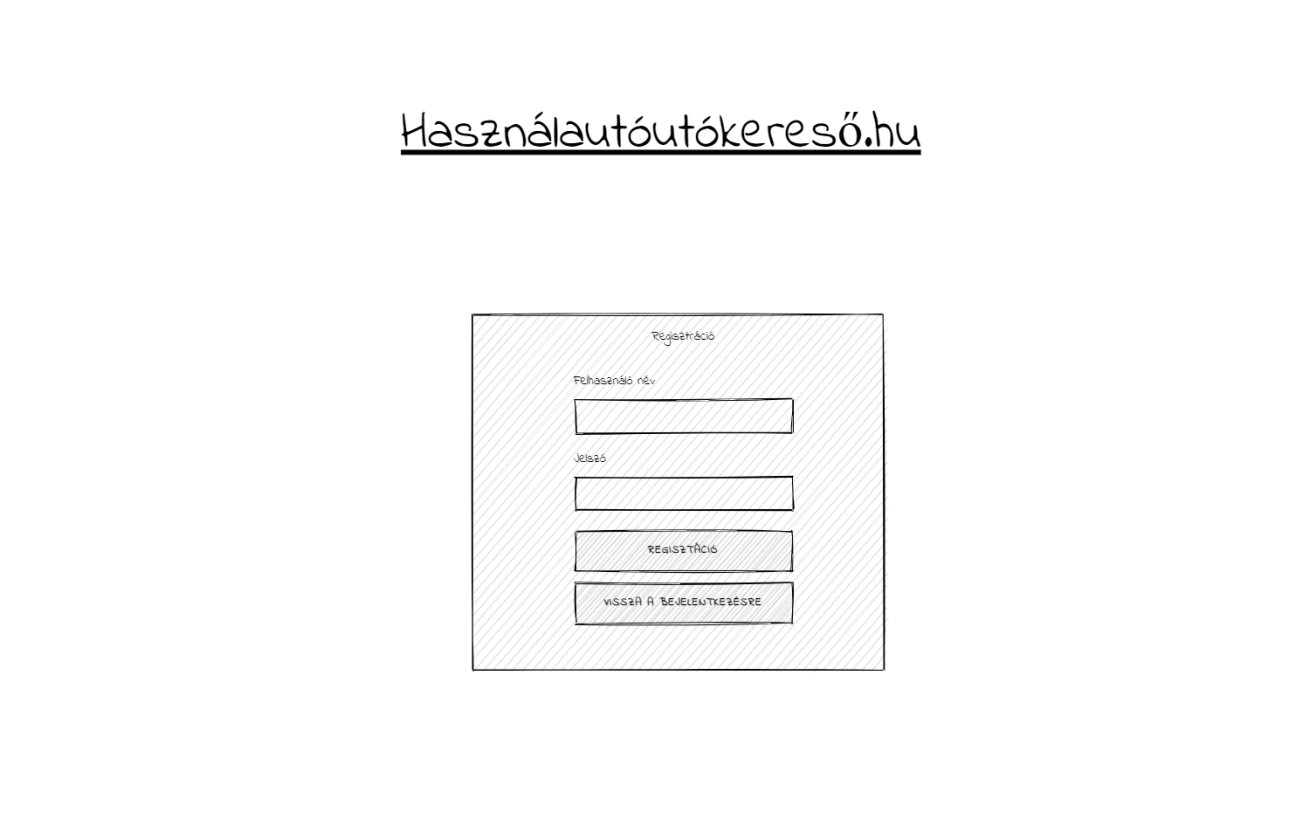
\includegraphics[scale=0.8]{images/register.png}}
\caption{Regisztráció}
\label{fig:Regisztráció}
\end{figure}

\newpage
\subsection{Főoldal}

A főoldalon látunk egy szűrő felületet, ahol ki lehet választani, hogy milyen márkájú és modellű autót milyen üzemanyag használattal, milyen évjárat és hengerűrtartalom között szeretnénk keresni. Van lehetőség az ár sáv megadására is (\ref{fig:Fooldal}. ábra).

Látunk, egy diagramot, ahol statisztikát tudunk megtekinteni az autókra keresések számáról egy adott időintervallumon belül. A vízszintes tengelyen az autómárkák neve lesz, a függőlegesen pedig a keresések száma.

\begin{figure}[h]
\centering
\fbox{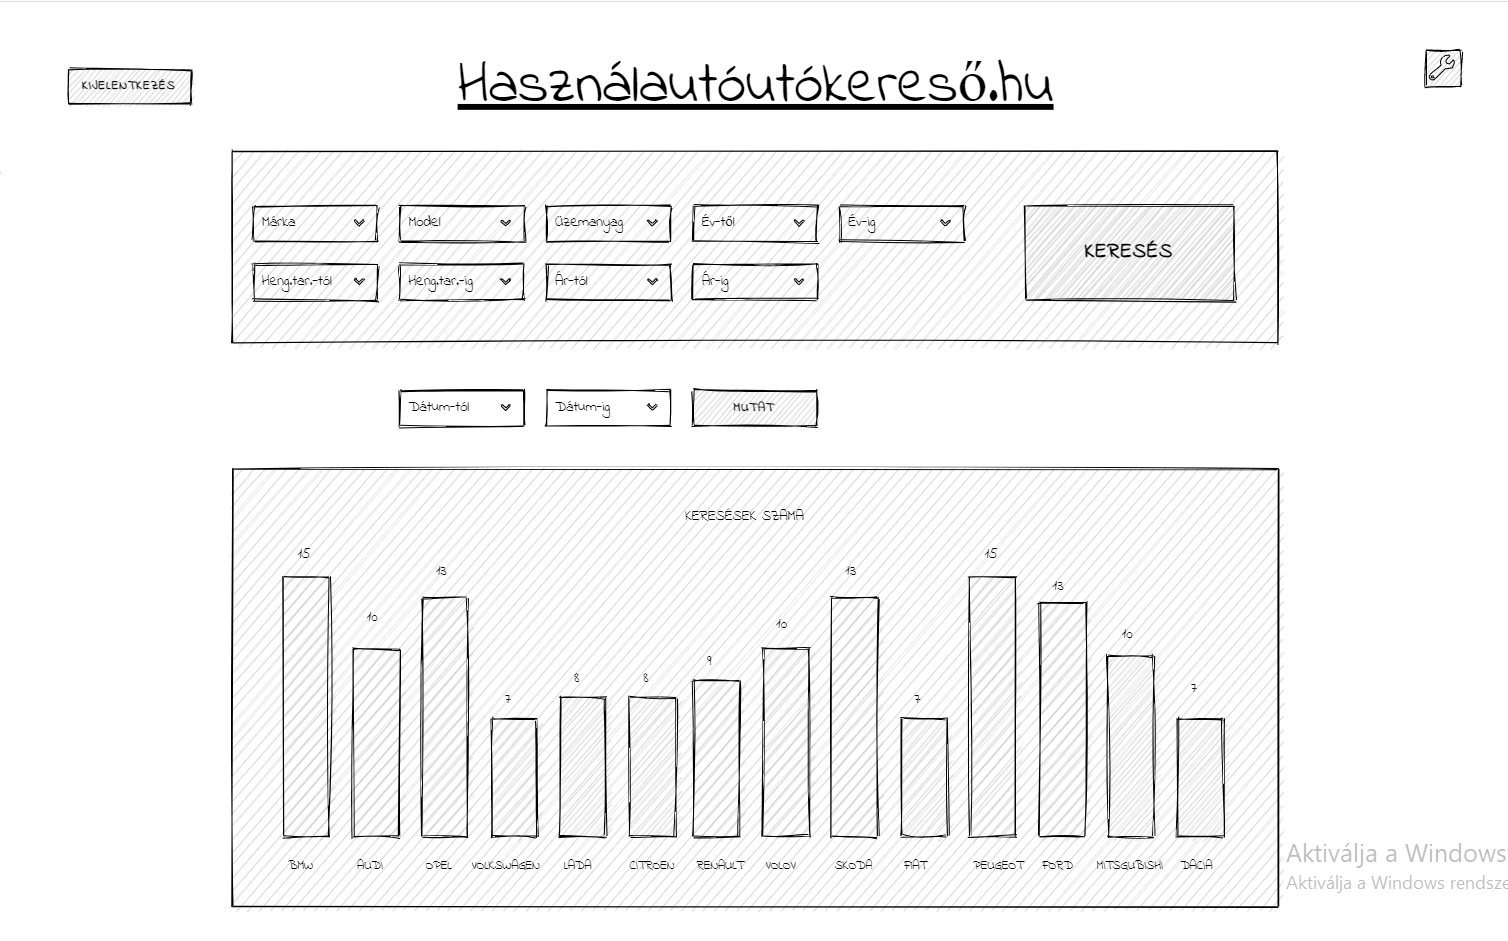
\includegraphics[scale=0.4]{images/Fooldal.png}}
\caption{Főoldal}
\label{fig:Fooldal}
\end{figure}

Van egy csavarkulcs ikon is, amit csak az \textit{admin} felhasználó lát. Ez a gomb az adminisztrátori felületre visz át.

\subsection{Találatok megtekintése}

A találati oldalon láthatjuk az autókat: egy képet az autóról, az alap információkat, mint évjárat, lóerő, vagy a köbcenti.

Ha megtaláljuk a megfelelő autót, akkor a "MEGNÉZEM" gombra kattintva meg is tudjuk tekinteni az autót (\ref{fig:Talalatok}. ábra).
\newpage

\begin{figure}[h]
\centering
\fbox{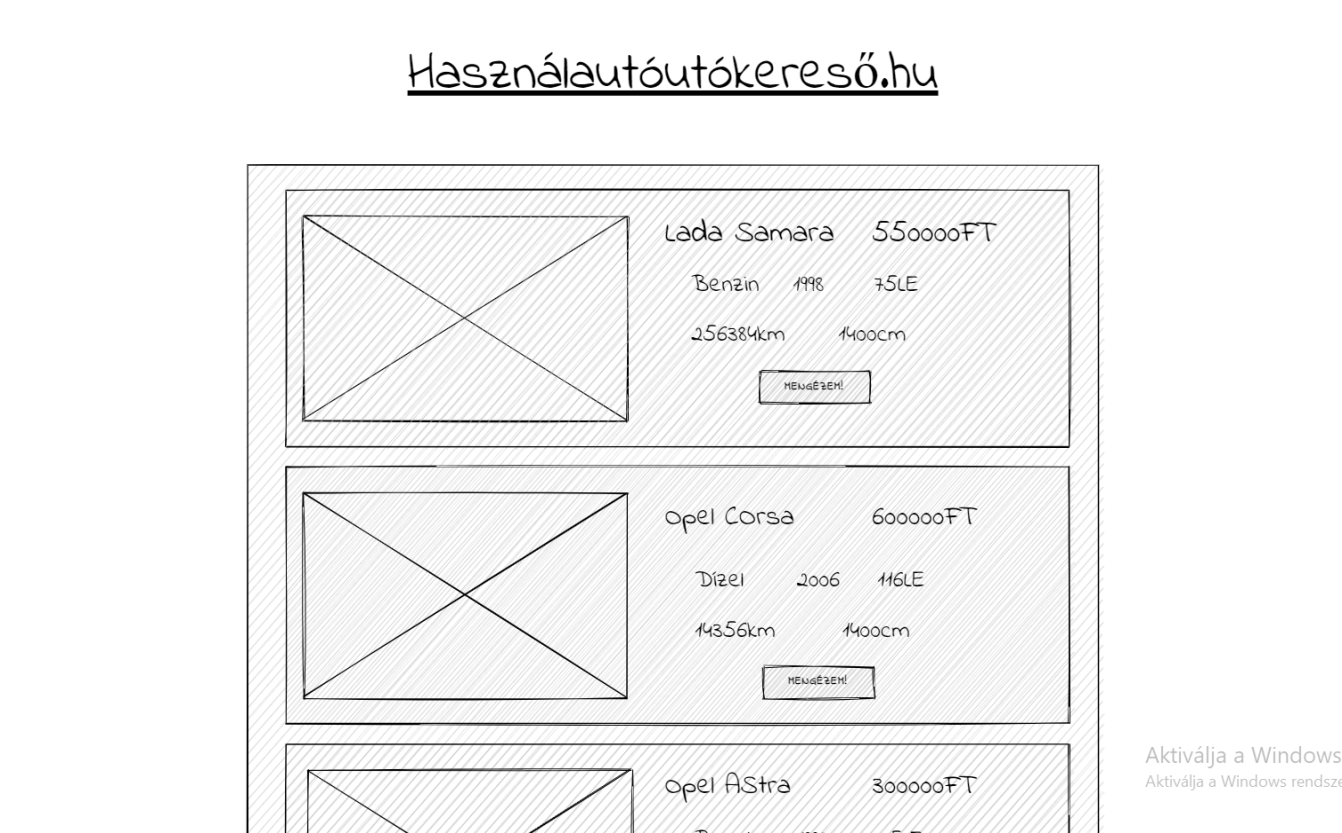
\includegraphics[scale=0.8]{images/Talalatok.png}}
\caption{Találati oldal}
\label{fig:Talalatok}
\end{figure}

\subsection{Adminisztrátori oldal}

Az Adminisztátori oldalon találunk egy táblázatot a felhasználókról, ami tartalmazza a felhasználó nevet és a jogosultságot. A jogosultságot itt tudjuk módosítani Admin és User között. Itt van lehetőség törölni a felhasználókat vagy az autók lekérdezésére a többi weboldalról (\ref{fig:Admin}. ábra).

\begin{figure}[h]
\centering
\fbox{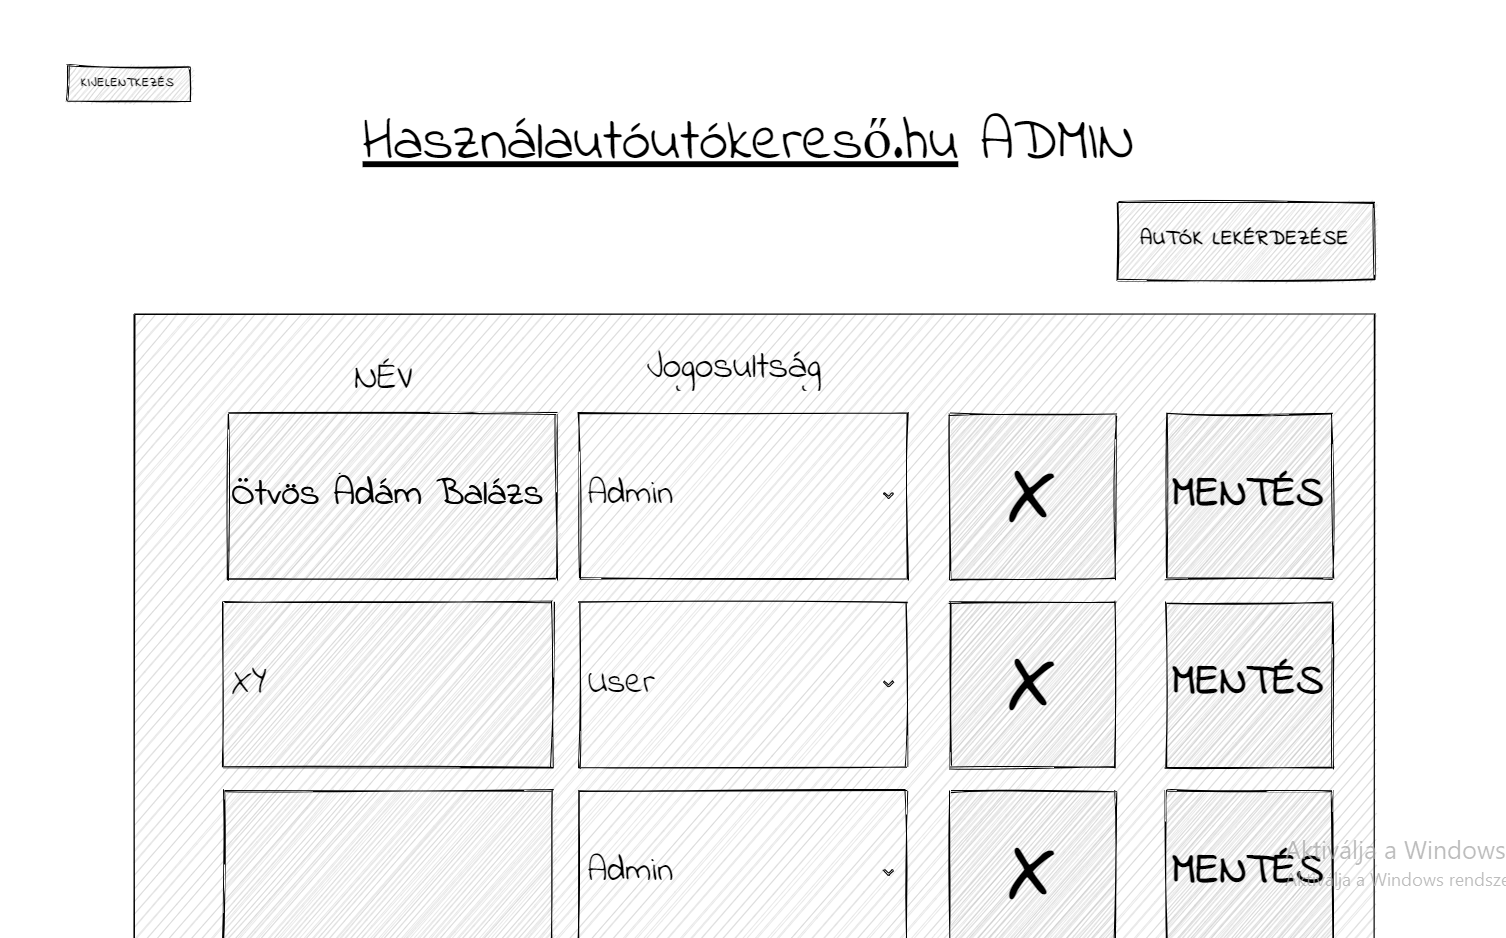
\includegraphics[scale=0.4]{images/Admin.png}}
\caption{Admin oldal}
\label{fig:Admin}
\end{figure}
\newpage

\Section{Adat táblák}

Az alkalmazás elkészítéséhez 3 darab táblára lesz szükség: a
felhasználók (\textit{users}), az autók (\textit{cars}) és a keresési adatok (\textit{search\_data}) táblára (\ref{fig:DataTable}. ábra).

\medskip
\textit{users} tábla:
\begin{itemize}
\item Itt lesznek eltárolva a felhasználó adatai a regisztráció után. Ilyen a jelszó, a felhasználónév és jogosultsága, hogy \textit{admin} vagy \textit{user}-e. A jogosultságot az \textit{admin} rangú felhasználó tudja változtatni.
\end{itemize}

\textit{cars} tábla:
\begin{itemize}
\item Az autók lekérdezése után itt tárolódnak az autók,  a hozzájuk tartozó adatok és a link, ami az autó hirdetésére vezet át
\end{itemize}

\textit{search\_data} tábla:
\begin{itemize}
\item Ez a tábla tárolja a márka nevét, és azt az időpontot, amikor csak egy adott márkájú autóra keresnek rá (márkára szűrve keresnek).
\end{itemize}
 
 \begin{figure}[h]
\centering
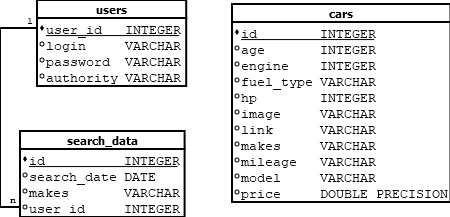
\includegraphics[scale=0.7]{images/Data_Table.png}
\caption{Adatbázis táblák}
\label{fig:DataTable}
\end{figure}

A \textit{users} és \textit{search\_data} tábla között egy-több kapcsolat lesz, mivel egy \textit{user}-hez több keresési előzmény is tartozhat, de egy kereséshez csak egy felhasználó.

A \textit{cars} tábla független lesz a többitől, mivel ide az adatok más oldalról lesznek letöltve, és így nem tartozik a \textit{users} táblához.

 
\Section{API-k megtervezése}
A programban használt API-ról, a definiált útvonalakról lesz szó ebben a szakaszban.
\begin{itemize}
\item /set

Ez egy \textit{POST} típusú kérés. Ha egy Admin frissíteni szeretné az autók tartalmát ez a végpont akkor fog meghívódni.
0 értéket fog vissza adni, amint befejezte a frissítést. A vissza adott érték \textit{String} típusú.
\item /get

Ez egy \textit{GET} típusú kérés. Ha egy felhasználó autóra akar keresni, akkor innen fognak lehívódni a megfelelő adatok.
RequestParam-étereket vár, és az autók listáját fogja vissza adni. Az összes paraméter \textit{String} típusú.
\item /getMakes

Ez egy \textit{GET} típusú kérés. Ez a végpont akkor fog meghívódni, amikor egy felhasználó márkára akar szűrni, hogy lássa milyen márkájú autók találhatóak a weboldalon.
Nem vár semmilyen értéket. A márkákat fogja vissza adni JSON formátumban.
\item /getModels

Ez egy \textit{GET} típusú kérés. Márka kiválasztása után automatikusan meghívódik azért, hogy tudjunk márkán belül modellekre is szűrni.
Egy márka paramétert vár és a hozzá tartozó modelleket fogja vissza adni JSON  formátumban. A paraméter \textit{String} típusú.
\item /dataGet

Ez egy \textit{GET} típusú kérés. Ha a felhasználó statisztikát szeretne nézni, akkor ez a végpont hívódik majd meg.
Egy kezdő és egy vég dátumot vár. Közötte lévő adatokat fogja vissza adni, JSON formátumban. A paraméterek \textit{String} típusúak.
\item /dataPost

Ez egy \textit{POST} típusú kérés. Autók lekérdezésének folyamatában fog meghívódni, és elmenti azt a márkát az adatbázisba azzal a dátummal, amikor szűrtek rá.
Egy RequestBody-t vár ami JSON formátumú és a felhasználónevet és a márkát fogja tartalmazni, \textit{String} típusúak. Üres értéket ad vissza.
\item /authenticate

Ez egy \textit{POST} típusú kérés. Ezen a végponton tud majd bejelentkezni a felhaszná-
ló.
Egy RequestBody-t vár ami a felhasználónevet és jelszót tartalmazza, \textit{String} típusúak. A tokent és a felhasználó adatait adja vissza JSON formátumban.
\item /register

Ez egy \textit{POST} típusú kérés. Regisztráláskor ide küldi majd el a felhasználó adatait a kliens.
Egy RequestBody-t vár ami a felhasználónevet és jelszót tartalmazza, \textit{String} típusúak. 0, 1, 2-es értékekkel térhet vissza. A visszatérés értéke 0, ha sikeres a regisztráció, 1, ha már létezik az adott nevű felhasználó, és 2, ha valamelyik adat nincs megadva.  
\item /users

Ez egy \textit{GET} típusú kérés. Itt tudjuk majd lekérdezni az összes felhasználót, a hozzá tartózó neveket és jogosultságokat.
A felhasználók listáját adja vissza JSON formátumban. Az adatok \textit{String} típusúak.
\item /userDelete

Ez egy \textit{DELETE} típusú kérés. Ennél a végpontnál tudunk majd felhasználót törölni.
Egy RequestParam-étert vár ami a törölni kívánt felhasználó nevét tartal-
mazza, típusa \textit{String}. Üres értéket ad vissza.
\item /userUpdate

Ez egy \textit{PUT} típusú kérés. Ennél  a végpontál tudjuk majd változtatni a felhasználó jogosultságát.
Egy RequestBody-t vár ami a felhasználónevet és az új jogosultsá-
got tartalmazza. JSON formátumban kapja meg az adatokat, amik \textit{String} típusú-
ak. Üres értéket ad vissza.

\end{itemize}









